\chapter{Configuração Final da Aeronave}
\label{cap:aeronave}

Com base no projeto conceitual e nos dimensionamentos e análises desenvolvidos durante o projeto preliminar, apresenta-se a configuração final proposta para a aeronave. O projeto resultante corresponde a uma aeronave regional turboélice, de asa alta, trem de pouso triciclo retrátil e empenagens convencionais, destinada ao transporte regional de passageiros e à operação adaptável para transporte de cargas.

As vistas apresentadas nas Figuras \ref{vista_lateral_aeronave}, \ref{vista_superior_aeronave} e \ref{vista_frontal_aeronave} sintetizam a configuração externa final da aeronave. Ressalta-se que todas as cotas indicadas nas vistas estão em milímetros.

\begin{figure}[H]
    \centering
    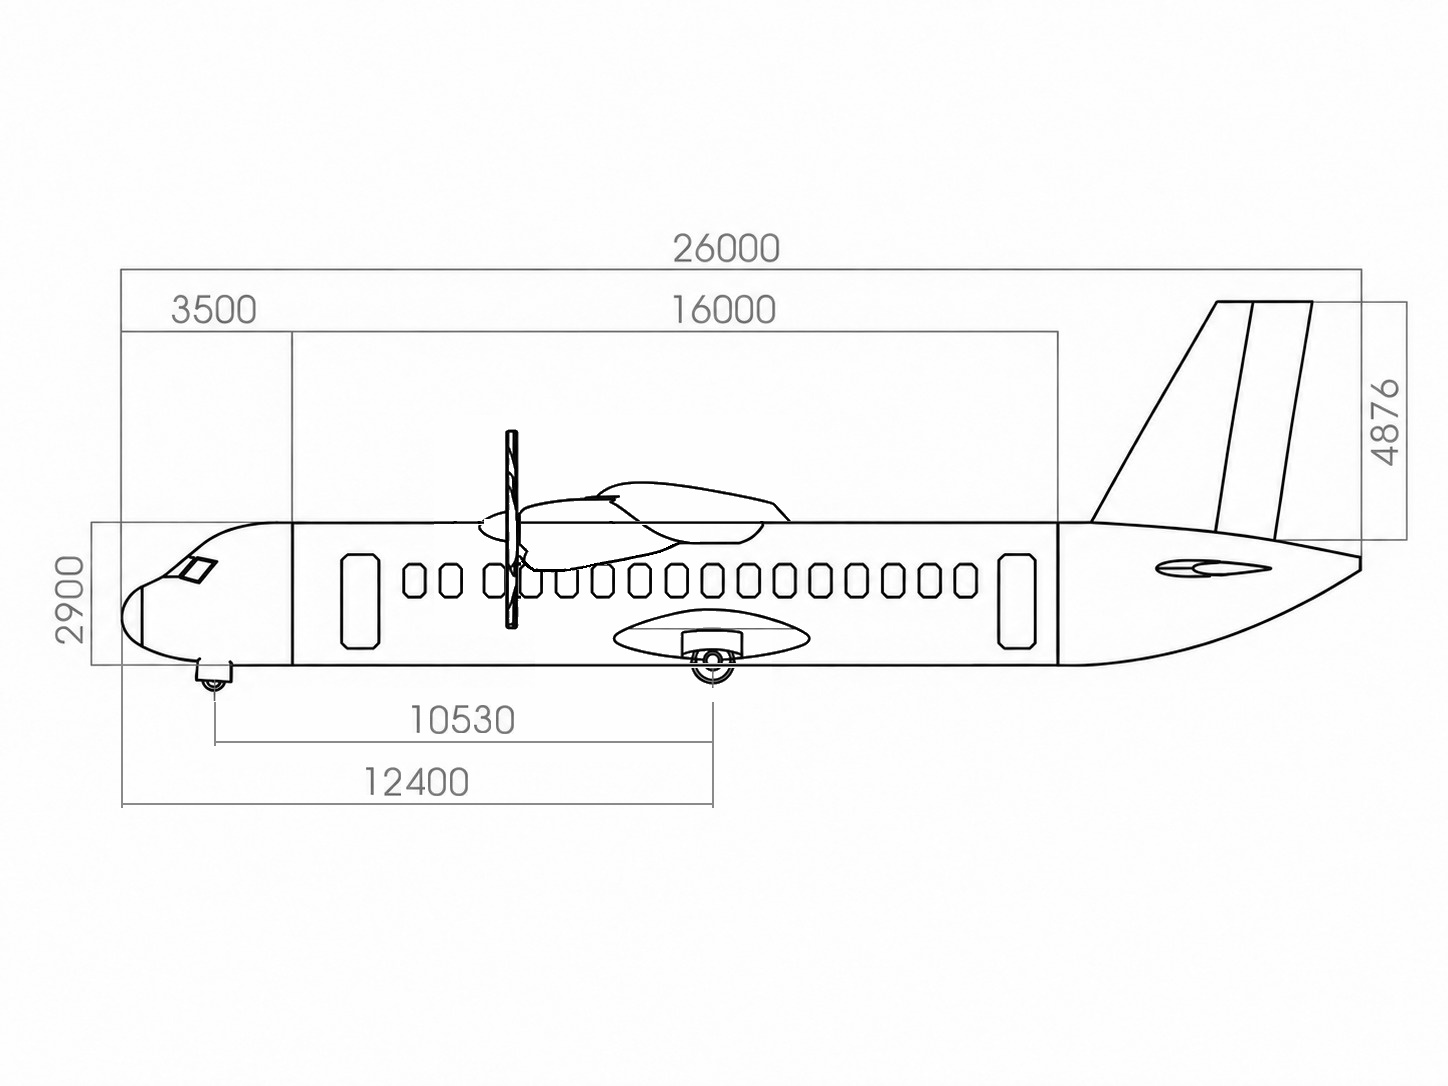
\includegraphics[width=0.92\textwidth]{Images-CG/VistaLateral.jpeg}
    \caption{Vista lateral da configuração final da aeronave.}
    \label{vista_lateral_aeronave}
\end{figure}

\begin{figure}[H]
    \centering
    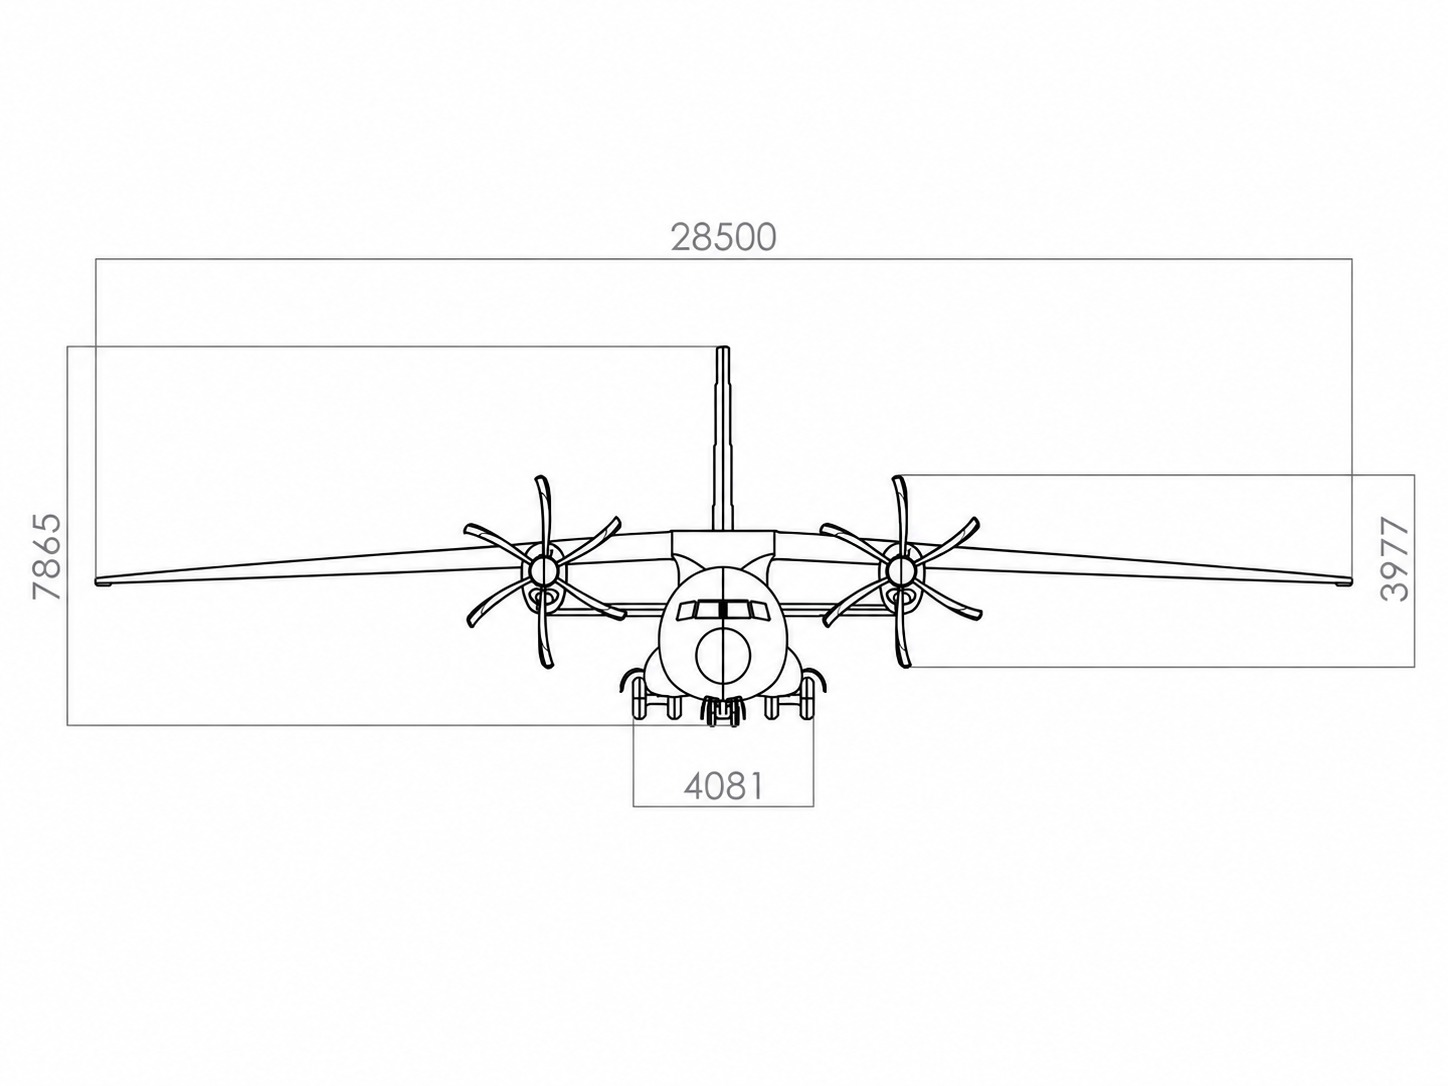
\includegraphics[width=0.92\textwidth]{Images-3-ProjetoDetalhado/VistaFrontal.jpeg}
    \caption{Vista frontal da configuração final da aeronave.}
    \label{vista_frontal_aeronave}
\end{figure}

\begin{figure}[H]
    \centering
    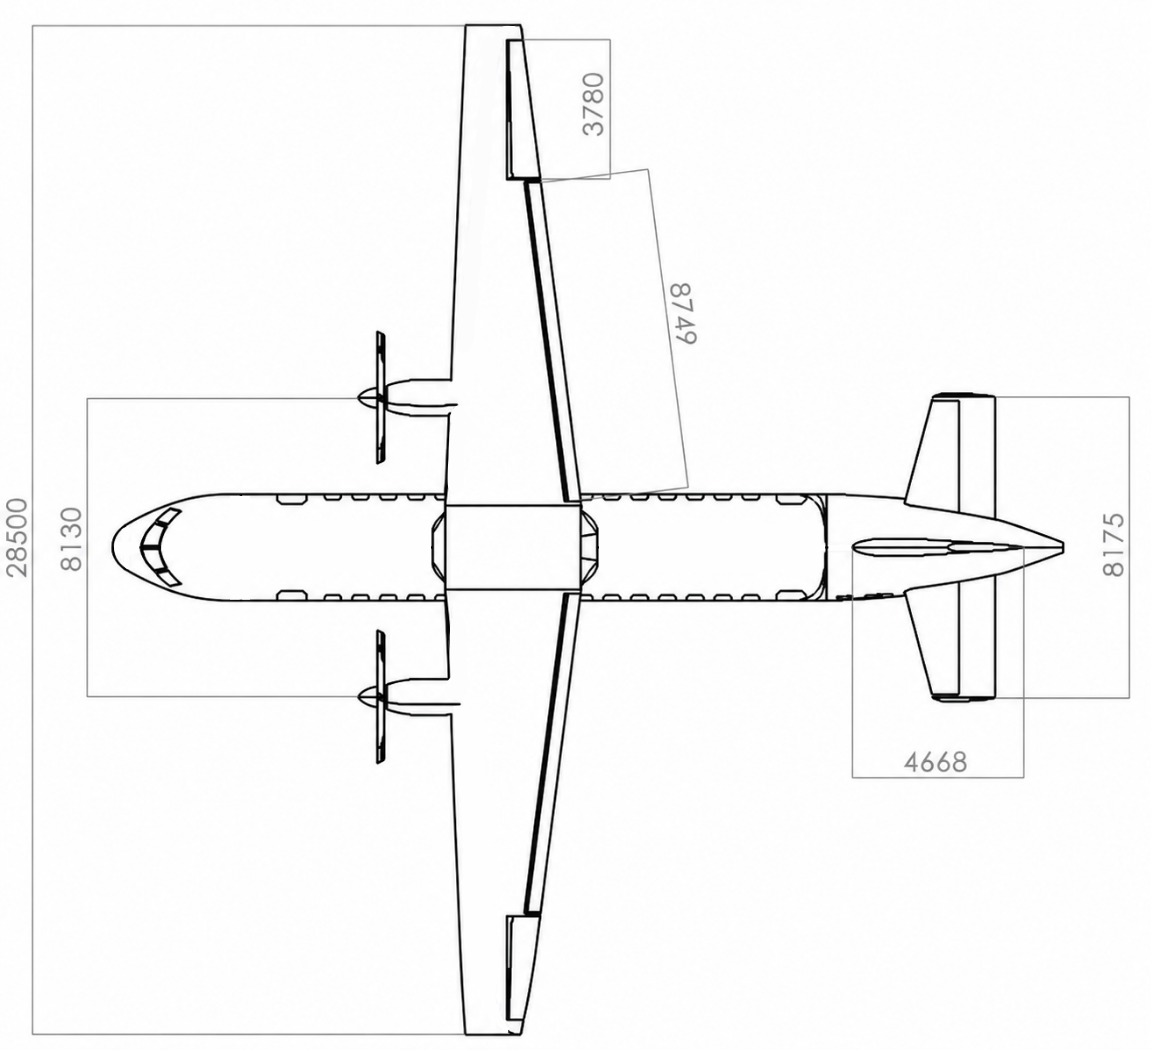
\includegraphics[width=0.8\textwidth]{Images-3-ProjetoDetalhado/VistaSuperior.jpeg}
    \caption{Vista superior da configuração final da aeronave.}
    \label{vista_superior_aeronave}
\end{figure}

Imagens adicionais da aeronave, contemplando outras perspectivas da configuração final, são apresentadas no Anexo.



\clearpage

\section{Resumo Técnico da Aeronave}
\label{sec:resumo_tecnico}

Abaixo são apresentados os principais parâmetros de projeto da aeronave.

% --- TABELA 1: VISÃO GERAL ---
\subsection{Visão Geral e Perfil de Missão}
\begin{table}[htbp]
\centering
\small
\begin{tabularx}{\textwidth}{lX}
\toprule
\textbf{Parâmetro} & \textbf{Especificação} \\
\midrule
Tipo de Aeronave & Transporte Regional (Passageiros e Cargas) \\
Arquitetura & Asa Alta, Empenagem Convencional, Trem de Pouso Triciclo Retrátil \\
Configuração de Passageiros & 64 passageiros (Arranjo 2+2, Pitch de 30 in / 762 mm) \\
Configuração de Cargas & \textit{Quick Change} (Trilhos estruturais, compatível com Paletes IATA PLA) \\
Tripulação de Voo & 2 Pilotos (\textit{Glass Cockpit} com 5 displays LCD) \\
\bottomrule
\end{tabularx}
\caption{Visão geral e perfil de missão da aeronave.}
\label{tab:visao_geral}
\end{table}


% --- TABELA 2: PESOS ---
\subsection{Pesos e Capacidades}
\begin{table}[htbp]
\centering
\small
\begin{tabularx}{\textwidth}{lX}
\toprule
\textbf{Parâmetro} & \textbf{Valor} \\
\midrule
Peso Máximo de Decolagem (MTOW) & 22.680 kgf (50.000 lb) \\
Peso Máximo de Pouso (MLW) & 22.350 kgf (49.273 lb) \\
Peso Máximo Zero Combustível (MZFW) & 19.592 kgf (43.193 lb) \\
Peso Vazio Operacional (OEW) & 13.512 kgf (29.789 lb), com tripulação e \textit{catering} \\
Peso Vazio ($W_E$) & 13.064 kgf (28.801 lb) \\
Carga Paga Máxima & 6.080 kgf (64 passageiros de 84 kg e 11 kg de bagagem cada) \\
Combustível com Carga Paga Máxima & 3.088 kgf (6.808 lb) \\
Capacidade de Combustível & 4.990 kgf (11.000 lb) \\
Envelope de CG & 17,9\% a 45,9\% da CMA (10,79 m a 11,56 m do nariz) \\
\bottomrule
\end{tabularx}
\caption{Pesos limites e capacidades estruturais.}
\label{tab:pesos_capacidades}
\end{table}

% --- TABELA 3: PROPULSÃO ---
\subsection{Grupo Motopropulsor}
\begin{table}[htbp]
\centering
\small
\begin{tabularx}{\textwidth}{lX}
\toprule
\textbf{Parâmetro} & \textbf{Especificação} \\
\midrule
Motores & 2x Pratt \& Whitney PW127M (Turboélice) \\
Potência Máxima (por motor) & 2.475 shp (Total Instalada: 4.950 shp) \\
Hélices & Hamilton Standard 568F (6 pás, passo variável) \\
Carga de Potência ($W/P$) & 4,58 kg/shp \\
\bottomrule
\end{tabularx}
\caption{Especificações do grupo motopropulsor.}
\label{tab:propulsao}
\end{table}

\clearpage

% --- TABELA 4: GEOMETRIA ---
\subsection{Dimensões Principais e Geometria}
\begin{table}[htbp]
\centering
\small
\begin{tabularx}{\textwidth}{llX}
\toprule
\textbf{Componente} & \textbf{Parâmetro} & \textbf{Valor} \\
\midrule
\textbf{Fuselagem} & Comprimento Total & 26,00 m \\
                   & Dimensões Internas da Cabine & 16,00 m (Comp.) $\times$ 2,60 m (Larg.) $\times$ 1,93 m (Alt.) \\
\midrule
\textbf{Asa}       & Envergadura ($b$) / Área ($S$) & 28,50 m / 74,10 m$^2$ \\
                   & Corda Média Aerodinâmica ($\bar{c}$) & 2,75 m \\
                   & Alongamento ($AR$) / Afilamento ($\lambda$) & 10,96 / 0,405 \\
                   & Perfis Aerodinâmicos & NACA 43016 (Raiz) / NACA 43009 (Ponta) \\
\midrule
\textbf{Empenagens} & Empenagem Horizontal & $S = 18,679$ m$^2$ / $b = 8,375$ m / NACA 0012 \\
                   & Empenagem Vertical & $S = 15,359$ m$^2$ / Altura = 4,925 m / NACA 0012 \\
\midrule
\textbf{Trem de Pouso} & Pneus (Principal / Nariz) & H34x10.0R16 (Radial) / 450x190-5 (Diagonal c/ Chine) \\
                       & Freios & Multidisco de Carbono (Cap. Térmica: 8,26 MJ) \\
\bottomrule
\end{tabularx}
\caption{Dimensões principais e características geométricas.}
\label{tab:geometria}
\end{table}

% --- TABELA 5: DESEMPENHO ---
\subsection{Desempenho e Envelope de Voo}
\begin{table}[htbp]
\centering
\small
\begin{tabularx}{\textwidth}{lX}
\toprule
\textbf{Parâmetro} & \textbf{Valor de Projeto} \\
\midrule
Velocidade de Cruzeiro de Projeto ($V_C$) & 230 kt EAS (\S 25.335) \\
Velocidade de Cruzeiro de Máximo Alcance & 193 kt TAS (357 km/h) a 20.000 ft \\
Velocidade Máxima em Cruzeiro & 247,1 kt (457,6 km/h) \\
Velocidade Máxima de Decolagem & 209,0 kt (387,0 km/h) \\
Velocidade de Estol ($V_S$) & 107,9 kt (Config. Pouso) / 125,8 kt (Config. Decolagem) \\
Distância Total de Decolagem & 1.102 m (3.614 ft) --- Ao nível do mar, ISA, MTOW \\
Distância Física de Pouso & 797 m (2.616 ft) --- Ao nível do mar, ISA, MLW \\
Teto de Serviço / Teto Absoluto & 24.438 ft (7.449 m) / 26.115 ft (7.960 m) \\
Alcance com Cabine Cheia e Reservas IFR & 925 NM (1.713 km); requisito: 800 NM \\
Autonomia do Trecho de Cruzeiro (cabine cheia) & 4,7 horas \\
Razão de Subida Máx. (Cruzeiro) & 1,23 m/s (aprox. 242 ft/min) \\
\bottomrule
\end{tabularx}
\caption{Parâmetros estimados de desempenho e operação.}
\label{tab:desempenho}
\end{table}

